

\documentclass[9pt]{beamer}
 \usepackage{multirow}
 \usepackage{natbib}
 \usepackage[normalem]{ulem}
\useunder{\uline}{\ul}{}
 \usepackage[utf8]{inputenc}
\usepackage{mathtools}
\usepackage{IEEEtrantools}
\usepackage[english]{babel}
\definecolor{maroon}{RGB}{153, 0, 0}
\usepackage[colorlinks=true, linkcolor= black, citecolor=maroon]{hyperref}


\usetheme{Madrid}
\definecolor{UBCblue}{rgb}{0.04706, 0.13725, 0.26667} % UBC Blue (primary)


\usecolortheme[named=UBCblue]{structure}

\usepackage{booktabs}
\let\olditem\item
\renewcommand{\item}{%
\olditem\vspace{\fill}} 
\usepackage{graphicx}
\usepackage{xfrac}
\usepackage{amsmath,amssymb,hyperref,array,xcolor,multicol,verbatim,mathpazo}




\title{Measuring the Natural Rate of Interest  in Brazil and identifying its drivers: a DSGE Perspective}
\subtitle{} 
\author[Alves, R. (EESP-FGV)]{Renan Alves}
{Orientador: Dr. Marcel Bertini Ribeiro \\
Coorientador: Dr. Marcelo Kfoury 
}
\date{\today}

\begin{document}
\setbeamertemplate{caption}{\raggedright\insertcaption\par}
\maketitle


%%%%%%%%%%%%%%%%%%%%%%%%%%%%%%%%%%%%%%%%%%%%%%%%%%%%%%%%%%%%%%%%%%%%%%%%%%%%
%%%%%%%%%%%%%%%%%%%%%%%%%%%%%%%%%%%%%%%%%%%%%%%%%%%%%%%%%%%%%%%%%%%%%%%%%%%%
\begin{frame}{Introduction}
\begin{itemize}

\item When measuring the effects of monetary policy conduct on the future behavior of inflation, it is prudent to construct a measure of monetary policy stance

\item This monetary policy indication measure is based on interest rates, it is the benchmark for the Central Bank. This benchmark is called the natural rate of interest

\item We refer to the natural interest rate and the natural level of the output (or potential), when prices and wages are flexible, according to \textcolor{red}{\citet{Woodford:2003}}

\item For the analysis of “inflationary or deflationary pressures”, the key variable to be measured is the gap between the natural rate of interest and the interest rate controlled by the Central Bank

\item It is a fundamental indicator of an appropriate monetary policy, especially in an inflation targeting regime. A good estimate of it and consequently of the interest rate gap, to indicate whether the monetary policy adopted was contractionary or expansionist


\end{itemize}
\end{frame}
%%%%%%%%%%%%%%%%%%%%%%%%%%%%%%%%%%%%%%%%%%%%%%%%%%%%%%%%%%%%%%%%%%%%%%%%%%%%
%%%%%%%%%%%%%%%%%%%%%%%%%%%%%%%%%%%%%%%%%%%%%%%%%%%%%%%%%%%%%%%%%%%%%%%%%%%%
\begin{frame}{Introduction}
\begin{itemize}
\item The aim of the paper is to estimate the natural rate of interest for the Brazilian economy and its drivers, using a New Keynesian model

\item We extended the articles of business cycles, for small open economy following \textcolor{red}{\citet{Gali:2005}} and \textcolor{red}{\citet{Lubik:2007}}, allowing preference shocks, technology shocks and external shocks.

\item The model incorporates the main characteristics of the DSGE models of small open economy and makes it possible to investigate how external shocks affect the natural rate in Brazil, during the post inflation target period

\item We evaluate the natural interest rate, using three different monetary policy rules. 
\begin{enumerate}
    \item Following the standard Taylor rule, with the central bank responding to deviation from inflation and the output gap
    
    \item The second the central bank responds to the natural interest rate and inflation
    
    \item Third rule is a combination of the previous two
\end{enumerate} 


\end{itemize}
\end{frame}
%%%%%%%%%%%%%%%%%%%%%%%%%%%%%%%%%%%%%%%%%%%%%%%%%%%%%%%%%%%%%%%%%%%%%%%%%%%%
%%%%%%%%%%%%%%%%%%%%%%%%%%%%%%%%%%%%%%%%%%%%%%%%%%%%%%%%%%%%%%%%%%%%%%%%%%%%
\begin{frame}{Preliminary Results}
\begin{itemize}
    \item Natural interest rate varies over the years and has dropped consistently
    
    \item Estimates are consistent for the three different monetary policy rules
    
    \item During the administration of Henrique Meirelles, the model in which the central bank responded to the neutral interest rate showed the lowest average natural interest
    
    \item Under the management of Alexandre Tombini, the lowest average neutral rate was estimated with the monetary policy rule that combines the Taylor rule with the Wickseliana
    
    \item While Ilan Goldfajn was president of the central bank, the lowest neutral interest rate was found when BC followed Taylor's rule
    
\end{itemize}


\end{frame}
%%%%%%%%%%%%%%%%%%%%%%%%%%%%%%%%%%%%%%%%%%%%%%%%%%%%%%%%%%%%%%%%%%%%%%%%%%%%
%%%%%%%%%%%%%%%%%%%%%%%%%%%%%%%%%%%%%%%%%%%%%%%%%%%%%%%%%%%%%%%%%%%%%%%%%%%%
\begin{frame}{How do economists estimate the Natural Interest Rate?}
\begin{itemize}

%\item The biggest problem found in the literature is that the neutral interest rate is not observed. Because of this, several econometric techniques are used to estimate the natural interest rate

\item  The first one relies on pure time-series methods – based on
multivariate time series models: \textcolor{red}{Hamilton et al. (2016)}, \textcolor{red}{Del Negro et al. (2018)} and \textcolor{red}{Christensen and Rudebusch (2019)} 

\item A second approach uses semistructural econometric models in which the natural rate is a latent variable that depend on the trend growth rate of potential output and a unit root process which captures other determinants: \textcolor{red}{\citet{LW:2003}}, \textcolor{red}{\citet{HLW:2017} },\textcolor{red}{\citet{Renne:2007}}, \textcolor{red}{\citet{Wynne:2018}}, \textcolor{red}{\citet{Us:2018}}, \textcolor{red}{\citet{Lewis:2017}}

\item The third class of articles uses structural models to estimate the neutral interest rate, DSGE models \textcolor{red}{\citet{Neiss:2003}},
\textcolor{red}{\citet{Edge:2008}}, \textcolor{red}{\citet{Lopez-Salido:2009}}, \textcolor{red}{\citet{Bjornland:2011}}, \textcolor{red}{\citet{Justiniano:2010} }, \textcolor{red}{Barsky et al. (2014)}, \textcolor{red}{\citet{Canzoneri:2015}}, \textcolor{red}{\citet{Curdia:2015}}, \textcolor{red}{\citet{Hristov:2016}}, \textcolor{red}{\citet{DelNegro:2017}},  \textcolor{red}{\citet{Neri:2018}}, \textcolor{red}{\citet{Grossman:2019}}, \textcolor{red}{\citet{Gali:2019}  }


\end{itemize}
\end{frame}
%%%%%%%%%%%%%%%%%%%%%%%%%%%%%%%%%%%%%%%%%%%%%%%%%%%%%%%%%%%%%%%%%%%%%%%%%%%%
%%%%%%%%%%%%%%%%%%%%%%%%%%%%%%%%%%%%%%%%%%%%%%%%%%%%%%%%%%%%%%%%%%%%%%%%%%%%
\begin{frame}{How do economists estimate the Natural Interest Rate in Brazil?}
\begin{itemize}

\item \textcolor{red}{\citet{Portugal:2009}}


\item \textcolor{red}{\citet{Barbosa:2016}}

\item \textcolor{red}{Neto and Candido (2018)}

\item \textcolor{red}{\citet{Moreira:2019}}

\item \textcolor{red}{\citet{Palma:2017}}



\end{itemize}
\end{frame}
%%%%%%%%%%%%%%%%%%%%%%%%%%%%%%%%%%%%%%%%%%%%%%%%%%%%%%%%%%%%%%%%%%%%%%%%%%%%
%%%%%%%%%%%%%%%%%%%%%%%%%%%%%%%%%%%%%%%%%%%%%%%%%%%%%%%%%%%%%%%%%%%%%%%%%%%%
\begin{frame}{Why use an open economy model?}
\begin{itemize}

\item \textcolor{red}{\citet{Barbosa:2016}} argues that the small open economy model is ideal for estimating the neutral interest rate in Brazil

\item \textcolor{red}{Perrelli (2019)} What would explain the decline in the neutral interest rate in Brazil?

\begin{itemize}
    \item Cyclic components: International interest rates, output gap, inflationary gap, credit to the private sector/GDP
    
    \item Fiscal components: BNDES loans, Government consumption, Public debt/GDP, Sovereign risk
    
    \item Structural components: Demography e.g \textcolor{red}{\citet{Ferrero:2016}}
\end{itemize}

\end{itemize}
\end{frame}

%%%%%%%%%%%%%%%%%%%%%%%%%%%%%%%%%%%%%%%%%%%%%%%%%%%%%%%%%%%%%%%%%%%%%%%%%%%%
%%%%%%%%%%%%%%%%%%%%%%%%%%%%%%%%%%%%%%%%%%%%%%%%%%%%%%%%%%%%%%%%%%%%%%%%%%%%
\begin{frame}{Model}
\begin{itemize}

\item \textcolor{red}{Gali and Monacelli (2005)} and \textcolor{red}{Lubik and Schorfheide (2007)}. It looks like \textcolor{red}{Gali (2015)}

\item IS Curve for small open economy:

\begin{equation*}
    x_t = E_t(x_{t+1}) - \frac{1}{(1-\alpha)\tau_{\alpha}}\left(i_t - E_t(\pi_{t+1}) - r_t^{n} \right)
\end{equation*}

$\tau_{\alpha} = \frac{1}{\tau + \alpha(2 - \alpha)(\eta - \tau)}$.

\item The Output Gap $x_t = y_{A,t} - y_{A,t}^{n}$ and the natural interest rate $r_t^{n}$.

\item The potential output of the domestic economy $y_{A,t}^{n}$ depends on the stationarized rest-of-the-world output  $y_{A,t}^{f}$ as follows: $y_{A,t}^{n} = - \Gamma_{*}y_{A,t}^{f} $.

onde $\Gamma_{*}=1-\sigma^{-1} \tau_{\alpha} / \sigma^{-1} \tau_{\alpha}+\sigma^{-1} \varphi$


\end{itemize}
\end{frame}
%%%%%%%%%%%%%%%%%%%%%%%%%%%%%%%%%%%%%%%%%%%%%%%%%%%%%%%%%%%%%%%%%%%%%%%%%%%%
%%%%%%%%%%%%%%%%%%%%%%%%%%%%%%%%%%%%%%%%%%%%%%%%%%%%%%%%%%%%%%%%%%%%%%%%%%%%
\begin{frame}{Modelo}
\begin{itemize}
\item The natural interest rate $r_t^{n}$ evolves according to:
\begin{equation*}
    r_t^{n} = E_t(\Delta \varepsilon_{t+1}^{c}) + \left( \frac{1 + \phi}{1 + \tau \phi} \right)E_t(z_{t+1}) + \left[\frac{1}{\tau} -(1 - \alpha)\tau_{\alpha}(\Gamma_{*}+1)   \right]E_t(\Delta y_{A,t+1}^{f})
\end{equation*}

\item preference shock: $\varepsilon_{t+1}^{c}$ and domestic technology
growth shock $z_t = ln\left( \frac{A_t}{A_{t-1}} \right)$.

\item The New Keynesian Phillips Curve:

\begin{equation*}
    \pi_t = \beta E_t(\pi_{t+1} ) + \alpha \beta E_t(q_{t+1}) - \alpha \Delta q_t + (\tau_{\alpha} + \phi) \kappa x_t + u_t
\end{equation*}

\item The terms of trade, $q_t$. CPI inflation as follows $\pi_t = \Delta s_t + (1 - \alpha) \Delta q_t + \pi_t^{f} $. $\pi_t^{f}$ is world inflation which we treat as an unobservable and assume it follows an  AR(1)


\end{itemize}
\end{frame}
%%%%%%%%%%%%%%%%%%%%%%%%%%%%%%%%%%%%%%%%%%%%%%%%%%%%%%%%%%%%%%%%%%%%%%%%%%%%
%%%%%%%%%%%%%%%%%%%%%%%%%%%%%%%%%%%%%%%%%%%%%%%%%%%%%%%%%%%%%%%%%%%%%%%%%%%%
\begin{frame}{Modelo}
\begin{itemize}
\item 3 differents Monetary Policy Rule.

\item A standard \textcolor{red}{Taylor (1993)}-type interest rate rule
\begin{equation*}
    i_t = \rho_i i_{t-1} + (1 - \rho_i)(\psi_{x}x_t + \psi_{\pi} \pi_t) + \varepsilon_{i,t}
\end{equation*}

\item The Wicksellian rule  (following \textcolor{red}{Cúrdia et al. (2015)}):
\begin{equation*}
    i_t = \rho_i i_{t-1} + (1 - \rho_i)(r_t^{n} + \psi_{\pi} \pi_t) + \varepsilon_{i,t}
\end{equation*}

\item With a more general rule Taylor and Wicksellian rule  (following \textcolor{red}{Cúrdia et al. (2015)}):
\begin{equation*}
    i_t = \rho_i i_{t-1} + (1 - \rho_i)(r_t^{n} + \psi_{x}x_t + \psi_{\pi} \pi_t) + \varepsilon_{i,t}
\end{equation*}

\item The terms of growth rates $\Delta q_t = \tau_{\alpha}(\Delta y_{A,t}^{f} - \Delta y_{A,t})$.

\item The growth rate of the terms of trade follows an AR(1): $\Delta q_t = \rho_q \Delta q_{t-1} + \varepsilon_{q,t}$.


\end{itemize}
\end{frame}
%%%%%%%%%%%%%%%%%%%%%%%%%%%%%%%%%%%%%%%%%%%%%%%%%%%%%%%%%%%%%%%%%%%%%%%%%%%%
%%%%%%%%%%%%%%%%%%%%%%%%%%%%%%%%%%%%%%%%%%%%%%%%%%%%%%%%%%%%%%%%%%%%%%%%%%%%
\begin{frame}{Data Description}
\begin{itemize}
    \item The data used are quartely series from 2000Q1 to 2019Q4
    
    \item We use observations on real output growth, inflation, nominal interest rates, exchange rate changes, and terms of trade growth. Foreign variables: output and inflation All series are demeaned prior to estimation
    
    \begin{itemize}
        \item 	Nominal exchange rate R$/US$ - BACEN - $s_t$
        
        \item 	Terms of trade – FUNCEX - $q_t$
        
        \item 	Real domestic output – IBGE – $y_t$
        
        \item 	Domestic inflation – IBGE - $\pi_t$
        
        \item 	Nominal Interest rate: annualized Selic rate $(\%)$ – BACEN - $i_t$
        
        \item 	US inflation – FRED (Fed St. Louis) -  $\pi_t^{*}$
        
        \item US output– FRED (Fed St. Louis) -  $y_t^{*}$
    \end{itemize}
    
    
\end{itemize}
\end{frame}
%%%%%%%%%%%%%%%%%%%%%%%%%%%%%%%%%%%%%%%%%%%%%%%%%%%%%%%%%%%%%%%%%%%%%%%%%%%%
%%%%%%%%%%%%%%%%%%%%%%%%%%%%%%%%%%%%%%%%%%%%%%%%%%%%%%%%%%%%%%%%%%%%%%%%%%%%
\begin{frame}{Bayesian Econometric - Priors}
\begin{figure}[H]
\centering
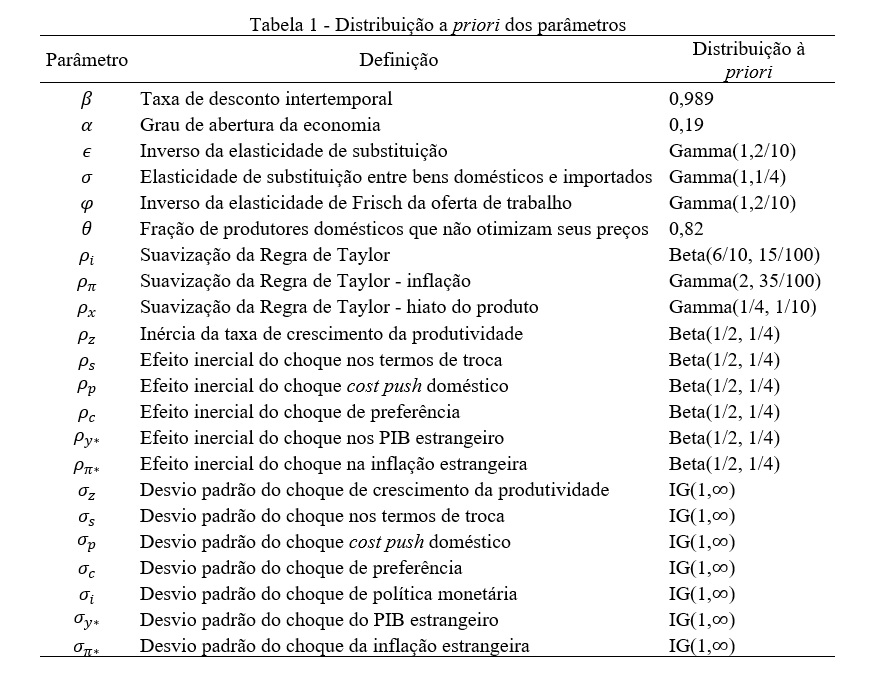
\includegraphics[scale=0.55]{Tabelaprioris.jpg}
%\caption {\tiny Taxa Natural de Juros}
\end{figure}


\end{frame}
%%%%%%%%%%%%%%%%%%%%%%%%%%%%%%%%%%%%%%%%%%%%%%%%%%%%%%%%%%%%%%%%%%%%%%%%%%%%
%%%%%%%%%%%%%%%%%%%%%%%%%%%%%%%%%%%%%%%%%%%%%%%%%%%%%%%%%%%%%%%%%%%%%%%%%%%%
\begin{frame}{Results}
\begin{itemize}
    \item Regra de Taylor
\end{itemize}
\begin{figure}[H]
\centering
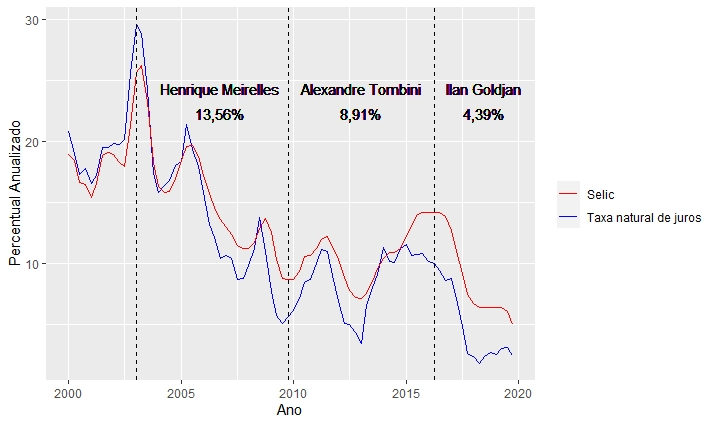
\includegraphics[scale=0.60]{ModeloA.jpeg}
%\caption {\tiny Taxa Natural de Juros}
\end{figure}

\end{frame}
%%%%%%%%%%%%%%%%%%%%%%%%%%%%%%%%%%%%%%%%%%%%%%%%%%%%%%%%%%%%%%%%%%%%%%%%%%%%
%%%%%%%%%%%%%%%%%%%%%%%%%%%%%%%%%%%%%%%%%%%%%%%%%%%%%%%%%%%%%%%%%%%%%%%%%%%%
\begin{frame}{Results}
\begin{itemize}
    \item Regra Wickseliana
\end{itemize}
\begin{figure}[H]
\centering
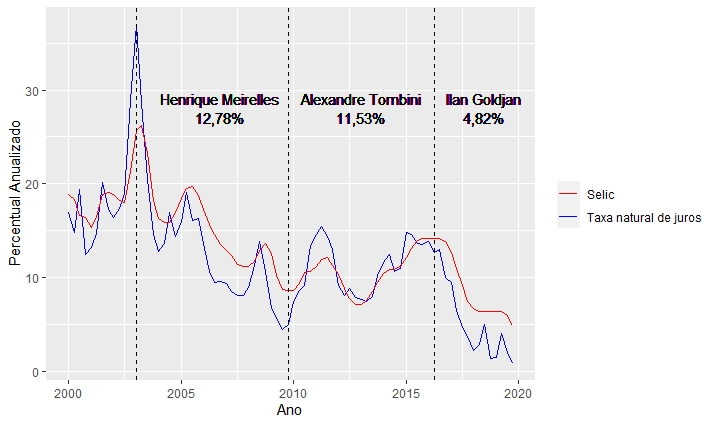
\includegraphics[scale=0.60]{ModeloB.jpeg}
%\caption {\tiny Taxa Natural de Juros}
\end{figure}

\end{frame}
%%%%%%%%%%%%%%%%%%%%%%%%%%%%%%%%%%%%%%%%%%%%%%%%%%%%%%%%%%%%%%%%%%%%%%%%%%%%
%%%%%%%%%%%%%%%%%%%%%%%%%%%%%%%%%%%%%%%%%%%%%%%%%%%%%%%%%%%%%%%%%%%%%%%%%%%%
\begin{frame}{Results}
\begin{itemize}
    \item Regra Taylor + Wickseliana
\end{itemize}
\begin{figure}[H]
\centering
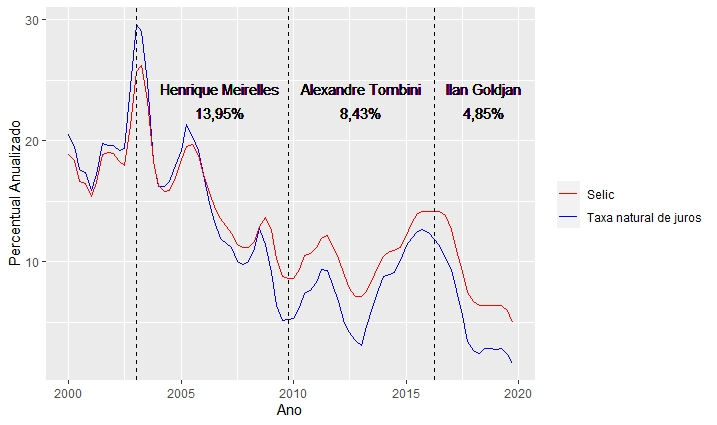
\includegraphics[scale=0.60]{ModeloC.jpeg}
%\caption {\tiny Taxa Natural de Juros}
\end{figure}

\end{frame}
%%%%%%%%%%%%%%%%%%%%%%%%%%%%%%%%%%%%%%%%%%%%%%%%%%%%%%%%%%%%%%%%%%%%%%%%%%%%
%%%%%%%%%%%%%%%%%%%%%%%%%%%%%%%%%%%%%%%%%%%%%%%%%%%%%%%%%%%%%%%%%%%%%%%%%%%%
\begin{frame}{Next  steps}
\begin{itemize}
    
    \item Extend the small open economy model by following the lines of \textcolor{red}{\citet{Adolfson:2007}}, which in turn extended the models of \textcolor{red}{\citet{Christiano:2005}} and \textcolor{red}{Altig et al. (2011)} into the open economy setting
    
    \item Adding a number of variables and frictions to the standard small open economy DSGE model structure
    
    \item  Investment (capital accumulation), exports and imports and their corresponding price deflators are added 
    
    \item In addition, the model includes a number of additional real and nominal frictions, such as investment adjustment costs, costly variation in the utilisation of capital and imperfect pass-through of import and export prices 
    
    \item Finally, add financial frictions, along the lines of work by \textcolor{red}{Bernanke et al. (1999)} and \textcolor{red}{Christiano et al. (2014)} 
    
    
\end{itemize}


\end{frame}
%%%%%%%%%%%%%%%%%%%%%%%%%%%%%%%%%%%%%%%%%%%%%%%%%%%%%%%%%%%%%%%%%%%%%%%%%%%%
%%%%%%%%%%%%%%%%%%%%%%%%%%%%%%%%%%%%%%%%%%%%%%%%%%%%%%%%%%%%%%%%%%%%%%%%%%%%



% ---------------------------------------
\begin{frame}[noframenumbering]

    
Appendix
\end{frame}

\begin{frame}{Firms}
\begin{itemize}
    \item \textbf{Domestic firms} \\
    
    \textbf{Final good producers} A final good producer transforms intermediate goods into a final homogeneous good, which in turn is used by households for either consumption or investment purposes
$$
    Y_{t}=\left[\int_{0}^{1} Y_{i, t} \frac{1}{\lambda_{d, t}} d i\right]^{\lambda_{d, t}}, 1 \leq \lambda_{d, t}<\infty
$$
$\lambda_{d, t}$ is a stochastic process determining the time-varying markup in the domestic goods market
$$
\lambda_{d, t}=\left(1-\rho_{\lambda_{d}}\right) \lambda_{d}+\rho_{\lambda_{d}} \lambda_{d, t-1}+\varepsilon_{t}^{\lambda_{d}}
$$
    
Profit maximisation by the final-good firm yields the demand
function for intermediate goods
$$
    Y_{i, t}=\left(\frac{P_{t}}{P_{i, t}}\right)^{\frac{\lambda_{d, t}}{\lambda_{d, t}-1}} Y_{t}
$$
    
\end{itemize}


\end{frame}
%%%%%%%%%%%%%%%%%%%%%%%%%%%%%%%%%%%%%%%%%%%%%%%%%%%%%%%%%%%%%%%%%%%%%%%%%%%%
%%%%%%%%%%%%%%%%%%%%%%%%%%%%%%%%%%%%%%%%%%%%%%%%%%%%%%%%%%%%%%%%%%%%%%%%%%%%
\begin{frame}{Firms}
\begin{itemize}
    \item \textbf{Domestic firms} \\
    
    \textbf{Intermediate good producers} A continuum of intermediate-good producers (indexed by $i,$ where $i \in[0,1]$ ) operate in a monopolistically competitive environment and produce differentiated goods according to the production function:
$$
Y_{i, t}=\varepsilon_{t}\left(K_{i, t}\right)^{\alpha}\left(z_{t} H_{i, t}\right)^{1-\alpha}-z_{t} \phi
$$
    \begin{itemize}
        
    \item $z_t$ and $\varepsilon_t$ are permanent and transitory technology shocks respectively  
    
    \item $K_{i,t}$, represents capital services stock which may differ from the physical capital stock since we allow for variable capital utilization in the model 
    
    \item $H_{i,t}$ is a homogenised labour input, and $\phi$ captures fixed costs that grow in line with technology 
    
   \item It is further assumed that the respective technology shocks follow autoregressive processes:
$$
    \begin{aligned}
    \frac{z_{t}}{z_{t-1}} &=\mu_{t}^{z} \\
    &=\left(1-\rho_{\mu^{z}}\right) \mu^{z}+\rho_{\mu^{z}} \mu_{t-1}^{z}+\epsilon_{t}^{z}
    \end{aligned}
$$
and
$$
    \hat{\varepsilon}_{t}=\rho_{\varepsilon} \hat{\varepsilon}_{t-1}+\varepsilon_{t}^{\varepsilon}
$$
where $\mu^{z}$ is the steady-state growth rate of technology, $E\left(\varepsilon_{t}\right)=1$ and $\hat{\varepsilon}_{t}=\left(\varepsilon_{t}-1\right) / 1 .$ since $\mu_{t}^{z}>1$

\end{itemize}
\end{itemize}


\end{frame}
%%%%%%%%%%%%%%%%%%%%%%%%%%%%%%%%%%%%%%%%%%%%%%%%%%%%%%%%%%%%%%%%%%%%%%%%%%%%
%%%%%%%%%%%%%%%%%%%%%%%%%%%%%%%%%%%%%%%%%%%%%%%%%%%%%%%%%%%%%%%%%%%%%%%%%%%%
\begin{frame}{Firms}
\begin{itemize}
    \item The intermediate firm rents capital services at the gross nominal rate $R_{t}^{k}$ and compensates the homogenous labour service at the nominal wage rate $W_{t} .$ Accordingly, the intermediate firm's cost minimisation problem is as follows:
$$
    \min _{K_{i, t}^{S}, H_{i, t}} W_{t} H_{i, t}+R_{t}^{k} K_{i, t}+\lambda_{t} P_{i, t}^{d}\left[Y_{i, t}-\varepsilon_{t}\left(K_{i, t}^{s}\right)^{\alpha}\left(z_{t} H_{i, t}\right)^{1-\alpha}+z_{t} \phi\right]
$$
Optimization of Equation with respect to $K_{i, t}$ and $H_{i, t}$ yields the familiar first-order conditions:
$$
    R_{t}^{k}=\alpha \lambda_{t} P_{i, t} z_{t}^{1-\alpha} \epsilon_{t}\left(K_{i, t}\right)^{\alpha-1} H_{i, t}^{1-\alpha}
$$
and
$$
    W_{t}=(1-\alpha) \lambda_{t} P_{i, t} z_{t}^{1-\alpha} \epsilon_{t}\left(K_{i, t}\right)^{\alpha} H_{i, t}^{-\alpha}
$$
that equate the marginal returns of capital and labour to the cost of their compensation
    
    
    
    
\end{itemize}


\end{frame}
%%%%%%%%%%%%%%%%%%%%%%%%%%%%%%%%%%%%%%%%%%%%%%%%%%%%%%%%%%%%%%%%%%%%%%%%%%%%
%%%%%%%%%%%%%%%%%%%%%%%%%%%%%%%%%%%%%%%%%%%%%%%%%%%%%%%%%%%%%%%%%%%%%%%%%%%%
\begin{frame}{Firms}
\begin{itemize}
    \item When combining Equations  the stationary real rental rate of capital is expressed as:
$$
r_{t}^{k}=\frac{\alpha}{1-\alpha} \bar{w}_{t} \mu_{t}^{z}\left(\frac{H_{t}}{k_{t}}\right)
$$
and real marginal cost as
$$
m c_{t}=\left(\frac{1}{1-\alpha}\right)^{1-\alpha}\left(\frac{1}{\alpha}\right)^{\alpha} \epsilon_{t}^{-1}\left(r_{t}^{k}\right)^{\alpha}\left(\bar{w}_{t}\right)^{1-\alpha}
$$
where the Lagrange multiplier in Equation $\lambda_{t} P_{i, t}^{d},$ is interpreted as nominal marginal cost $M C_{t}$
    
\item Because of the permanent technology shock and the unit-root in the price level, a number of variables are non-stationary as they contain a nominal and real stochastic trend. We follow \textcolor{red}{Altig et al. (2011)} and stationarize the variables in the following way
$$
    r_{t}^{k} \equiv \frac{R_{t}^{k}}{P_{t}}, \bar{w}_{t} \equiv \frac{W_{t}}{P_{t} z_{t}}, k_{t+1} \equiv \frac{K_{t+1}}{z_{t}} \text { and } \bar{k}_{t+1} \equiv \frac{\bar{K}_{t+1}}{z_{t}}
$$    
    
    
\end{itemize}


\end{frame}
%%%%%%%%%%%%%%%%%%%%%%%%%%%%%%%%%%%%%%%%%%%%%%%%%%%%%%%%%%%%%%%%%%%%%%%%%%%%
%%%%%%%%%%%%%%%%%%%%%%%%%%%%%%%%%%%%%%%%%%%%%%%%%%%%%%%%%%%%%%%%%%%%%%%%%%%%
\begin{frame}{Firms}
\begin{itemize}
    \item \textbf{Domestic firms setting} 
    \begin{itemize}
        \item It is assumed that intermediate-good firms set prices in a staggered manner as proposed by \textcolor{red}{Calvo (1983)}. In his model a firm gets the opportunity to adjust its price with a probability of $\left( 1 - \xi_{d} \right)$ in every period. The reoptimized price is $P_t^{new}$
        
        \item With probability $\xi_{d}$ the firm is not allowed to reoptimize, and its price in period $t+1$ is then updated according to the scheme $P_{t+1}=\left(\pi_{t}\right)^{\kappa_{d}}\left(\bar{\pi}_{t+1}^{c}\right)^{1-\kappa_{d}} P_{t},$ i.e. and the current inflation target, $\bar{\pi}_{t+1}^{c}$ where $\kappa_{d}$ is an indexation parameter 
        
        \item Thus, firm $i$ faces the following optimization problem when setting its price:
        
$$\begin{aligned}
    \max _{\tilde{P}_{t}^{new}} E_{t} \sum_{s=0}^{\infty}\left(\beta \xi_{d}\right)^{s} v_{t+s}\left\{\left[\left(\prod_{k=1}^{s} \pi_{t+k-1}\right)^{\kappa_{d}}\left(\prod_{k=1}^{s} \bar{\pi}_{t+k}^{c}\right)^{1-\kappa_{d}} \tilde{P}_{t}^{new}\right]\right.& Y_{i, t+s} \\
    \left.-M C_{i, t+s}\left(Y_{i, t+s}+z_{t+s} \phi\right)\right\} &
    \end{aligned}
$$    

    \item The New Keynesian Phillips curve for the domestic good:
$$
    \begin{aligned}
    \hat{\pi}_{t}-\hat{\tilde{\pi}}_{t}^{c} &=\frac{\beta}{1+\kappa_{d} \beta}\left(E_{t} \hat{\pi}_{t+1}-\rho_{\pi} \hat{\pi}_{t}^{c}\right)+\frac{\kappa_{d}}{1+\kappa_{d} \beta}\left(\hat{\pi}_{t-1}-\hat{\tilde{\pi}}_{t}^{c}\right)-\frac{\kappa_{d} \beta\left(1-\rho_{\pi}\right)}{1+\kappa_{d} \beta} \hat{\tilde{\pi}}_{t}^{c} \\
    &+\frac{\left(1-\xi_{d}\right)\left(1-\beta \xi_{d}\right)}{\left(1+\kappa_{d} \beta\right) \xi_{d}}\left(\hat{m} c_{t}+\hat{\lambda}_{t}^{d}\right)
    \end{aligned}
$$
    
    
    
\end{itemize}
    
\end{itemize}


\end{frame}
%%%%%%%%%%%%%%%%%%%%%%%%%%%%%%%%%%%%%%%%%%%%%%%%%%%%%%%%%%%%%%%%%%%%%%%%%%%%
%%%%%%%%%%%%%%%%%%%%%%%%%%%%%%%%%%%%%%%%%%%%%%%%%%%%%%%%%%%%%%%%%%%%%%%%%%%%
\begin{frame}{Firms}
\begin{itemize}
    \item \textbf{Importing firms} 
    \begin{itemize}
        \item There are two types of importing firms:  the importing consumption firm turns the homogeneous good into a differentiated consumption good $C_{i,t}^{m}$, while a differentiated investment good $I_{i,t}^{m}$ is created by the importing investment firm
        
        \item Both of these importing firms purchase a homogeneous good in the world market at the international price $P_t^{*}$

        \item As with domestic firms, it is assumed that importing firms face a \textcolor{red}{Calvo (1983)} probability when setting their price. Hence, importing consumption firms may change their price with probability $\left(1 - \xi_{m,c}\right)$ and investment firms with probability $\left(1 - \xi_{m,i}\right)$
        
        \item Firms who cannot reoptimise, index their price in period $t + 1$ to a combination of the previous period’s imported price inflation rate $\pi_t^{m,j}$ for  $j = \left\{c,i \right\}$ and the current inflation target $\bar{\pi}_{t+1}^{c}$ as follows: $P_{t+1}^{m, j}=\left(\pi_{t}^{m, j}\right)^{\kappa_{m, j}}\left(\bar{\pi}_{t+1}^{c}\right)^{1-\kappa_{m, j}} P_{t}^{m, j}$
        
        \item The consumption and investment importing firms face the following optimization problem, respectively:
        
$$\begin{array}{c}
    \max _{P_{new,t}^{m,j}} E_{t} \sum_{s=0}^{\infty}\left(\beta \xi_{m, j}\right)^{s} v_{t+s}\left\{\left[\left(\prod_{k=1}^{s} \pi_{t+k-1}^{m, j}\right)^{\kappa_{m, j}}\left(\prod_{k=1}^{s} \bar{\pi}_{t+k}^{c}\right)^{1-\kappa_{m, j}} P_{new,t}^{m, j}\right] M_{i, t+s}\right. \\
    \left.-S_{t+s} P_{t+s}^{*}\left(M_{i, t+s}+z_{t+s} \phi^{m, j}\right)\right\}
    \end{array}
$$
    

    
\end{itemize}
\end{itemize}

\end{frame}
%%%%%%%%%%%%%%%%%%%%%%%%%%%%%%%%%%%%%%%%%%%%%%%%%%%%%%%%%%%%%%%%%%%%%%%%%%%%
%%%%%%%%%%%%%%%%%%%%%%%%%%%%%%%%%%%%%%%%%%%%%%%%%%%%%%%%%%%%%%%%%%%%%%%%%%%%
\begin{frame}{Firms}
\begin{itemize}
    \item \textbf{Importing firms} 
    \begin{itemize}
        \item The final imported good can be expressed as a CES composite of the differentiated import goods: $M_{t}=\left[\int_{0}^{1}\left(M_{i, t}\right)^{\frac{1}{\lambda^{m, j}}} d i\right]^{\lambda_{t}^{m, j}}$
        
        \item The demand function faced by each importing firm i is given by: $M_{i, t}=\left(\frac{P_{i, t}^{m, j}}{P_{t}^{m, j}}\right)^{-\frac{\lambda_{t, j}^{m, j}}{\lambda_{t}^{m, j}-1}} M_{t}$ 
        
        \item  the time-varying markup for the imported consumption and investment goods is: $\lambda_{t}^{m, j}=\left(1-\rho_{\lambda^{m, j}}\right) \lambda^{m, j}+\rho_{\lambda^{m, j}} \lambda_{t-1}^{m, j}+\epsilon_{t}^{\lambda^{m, j}}$
        
        
        \item Phillips curve relations for the imported consumption and investment good:
$$\begin{aligned}
    \left(\widehat{\pi}_{t}^{m, j}-\widehat{\bar{\pi}}_{t}^{c}\right)=& \frac{\beta}{1+\kappa_{m, j} \beta}\left(\mathrm{E}_{t} \widehat{\pi}_{t+1}^{m, j}-\rho_{\pi} \widehat{\bar{\pi}}_{t}^{c}\right)+\frac{\kappa_{m, j}}{1+\kappa_{m, j} \beta}\left(\widehat{\pi}_{t-1}^{m, j}-\widehat{\bar{\pi}}_{t}^{c}\right) \\
    &-\frac{\kappa_{m, j} \beta\left(1-\rho_{\pi}\right)}{1+\kappa_{m, j} \beta} \widehat{\bar{\pi}}_{t}^{c}+\frac{\left(1-\xi_{m, j}\right)\left(1-\beta \xi_{m, j}\right)}{\xi_{m, j}\left(1+\kappa_{m, j} \beta\right)}\left(\widehat{m c}_{t}^{m, j}+\widehat{\lambda}_{t}^{m, j}\right)
    \end{aligned}
$$    

    \item $\widehat{m c}_{t}^{m, j} = \widehat{p}_t^{*} + \widehat{s}_t - \widehat{p}_t^{m,j}$ for $j = \left\{c,i \right\}$. The markup shocks, $\widehat{\lambda}_t^{m,j} $
    
    
    
    

\end{itemize}
\end{itemize}

\end{frame}
%%%%%%%%%%%%%%%%%%%%%%%%%%%%%%%%%%%%%%%%%%%%%%%%%%%%%%%%%%%%%%%%%%%%%%%%%%%%
%%%%%%%%%%%%%%%%%%%%%%%%%%%%%%%%%%%%%%%%%%%%%%%%%%%%%%%%%%%%%%%%%%%%%%%%%%%%
\begin{frame}{Firms}
\begin{itemize}
    \item \textbf{Exporting firms} 
    \begin{itemize}
        \item Exporting firms purchase the final good, differentiate it and then sell this continuum of differentiated xport goods to households abroad. The demand faced by the individual exporting firm is given by:
$$
    \tilde{X}_{i, t}=\left(\frac{P_{i, t}^{x}}{P_{t}^{x}}\right)^{-\frac{\lambda_{t}^{x}}{\lambda_{t}^{x}-1}} \tilde{X}_{t}
$$    
    \item where $P_t^{x}$ is the foreign currency price of exports, and the time-varying markup for the exporting firm is: $\lambda_{t}^{x}=\left(1-\rho_{\lambda^{x}}\right) \lambda^{x}+\rho_{\lambda^{x}} \lambda_{t-1}^{x}+\varepsilon_{t}^{\lambda^{x}}$
    
    \item In order to allow for incomplete exchange rate pass-through in the export market, we assume that export prices are sticky in the foreign currency. To model this we use the Calvo setup
    
    \item  The price in period t+1 is thus $P_{t+1}^{x}=\left(\pi_{t}^{x}\right)^{\kappa_{x}}\left(\bar{\pi}_{t+1}^{c}\right)^{1-\kappa_{x}} P_{t}^{x}$. The export firms maximize profits (denoted in the local currency) taking into account that there might not be a chance to optimally change the price: 
    

$$\begin{array}{c}
    \max _{P_{new,t}^{x}} E_{t} \sum_{s=0}^{\infty}\left(\beta \xi_{x, j}\right)^{s} v_{t+s}\left\{\left[\left(\prod_{k=1}^{s} \pi_{t+k-1}^{x}\right)^{\kappa_{x, j}}\left(\prod_{k=1}^{s} \bar{\pi}_{t+k}^{c}\right)^{1-\kappa_{x, j}} P_{new,t}^{x}\right] \tilde{X}_{i, t+s}\right. \\
    \left.-\frac{P_{t+s}}{S_{t+s}}\left(\tilde{X}_{i, t+s}+z_{t+s} \phi^{x}\right)\right\}
    \end{array}
$$

    
\end{itemize}
\end{itemize}

\end{frame}
%%%%%%%%%%%%%%%%%%%%%%%%%%%%%%%%%%%%%%%%%%%%%%%%%%%%%%%%%%%%%%%%%%%%%%%%%%%%
%%%%%%%%%%%%%%%%%%%%%%%%%%%%%%%%%%%%%%%%%%%%%%%%%%%%%%%%%%%%%%%%%%%%%%%%%%%%
\begin{frame}{Firms}
\begin{itemize}
    \item \textbf{Exporting firms} 
    \begin{itemize}
        \item The log-linearized first order condition of this problem implies that the aggregate export inflation is given by
        
$$\begin{aligned}
    \left(\widehat{\pi}_{t}^{x}-\widehat{\pi}_{t}^{c}\right)=& \frac{\kappa_{x}}{1+\beta \kappa_{x}}\left(\widehat{\pi}_{t-1}^{x}-\widehat{\pi}_{t}^{c}\right)+\frac{\beta}{1+\beta \kappa_{x}}\left(\mathrm{E}_{t} \widehat{\pi}_{t+1}^{x}-\rho_{\pi} \widehat{\pi}_{t}^{c}\right) \\
    &-\frac{\beta \kappa_{x}\left(1-\rho_{\pi}\right)}{1+\beta \kappa_{x}} \widehat{\pi}_{t}^{c}+\frac{\left(1-\beta \xi_{x}\right)\left(1-\xi_{x}\right)}{\xi_{x}\left(1+\beta \kappa_{x}\right)}\left(\widehat{m c}_{t}^{x}+\widehat{\lambda}_{x, t}\right)
\end{aligned}$$
    
    \item $\widehat{mc}_t^{x} = \widehat{p}_t - \widehat{s}_t - \widehat{p}_t^{x}$
    
    \item In the foreign economy, the exported good may either be used for consumption $C_t^{*}$ or investment $I_t^{*}$
    
    \item foreign demand for the (aggregate) domestic consumption good, $C_t^{x}$, is given by $C_{t}^{x}=\left[\frac{P_{t}^{x}}{P_{t}^{*}}\right]^{-\eta_{f}} C_{t}^{*}$
    
    \item foreign investment demand for the domestic good: $I_{t}^{x}=\left[\frac{P_{t}^{x}}{P_{t}^{*}}\right]^{-\eta_{f}} I_{t}^{*}$
    
\end{itemize}
\end{itemize}

\end{frame}
%%%%%%%%%%%%%%%%%%%%%%%%%%%%%%%%%%%%%%%%%%%%%%%%%%%%%%%%%%%%%%%%%%%%%%%%%%%%
%%%%%%%%%%%%%%%%%%%%%%%%%%%%%%%%%%%%%%%%%%%%%%%%%%%%%%%%%%%%%%%%%%%%%%%%%%%%
\begin{frame}{Households}
\begin{itemize}
    \item A continuum of infinitely-lived households (indexed by $j$, where $j \in [0,1]$) populate the domestic economy. 
    
    \item In every period, the $j^{th}$ household maximises expected lifetime utility according to following intertemporal utility
    function
    
    $$E_{0}^{j} \sum_{t=0}^{\infty} \beta^{t}\left[\zeta_{t}^{c} \ln \left(C_{j, t}-b C_{j, t-1}\right)-\zeta_{t}^{h} A_{L} \frac{\left(b_{j, t}\right)^{1+\sigma_{L}}}{1+\sigma_{L}}\right]$$
    
    $$\begin{array}{l}
\zeta_{t}^{c}=\rho_{c} \zeta_{t-1}^{c}+\varepsilon_{t}^{\zeta_c} \\
\zeta_{t}^{h}=\rho_{c} \zeta_{t-1}^{h}+\varepsilon_{t}^{\zeta_h}
\end{array}$$    

    \begin{itemize}
        \item \textbf{Consumption} The aggregate consumption basket from which households derive utility is given by the CES index: $C_{t}=\left[\left(1-\omega_{c}\right)^{\frac{1}{\eta_{c}}}\left(C_{t}^{d}\right)^{\frac{\eta_{c}-1}{n_{c}}}+\omega_{c}^{\frac{1}{\eta_{c}}}\left(C_{t}^{m}\right)^{\frac{\eta_{c}-1}{\eta_{c}}}\right]^{\frac{\pi_{c}}{\eta_{c}-1}}$
        
    \item the price index for the consumption basket (CPI) is: $P_{t}^{c}=\left[\left(1-\vartheta_{c}\right)\left(P_{t}^{d}\right)^{1-\eta_{c}}+\vartheta_{c}\left(P_{t}^{m, c}\right)^{1-\eta_{c}}\right]^{\frac{1}{1-\eta_{c}}}$
        
        
    \end{itemize}
    

\end{itemize}

\end{frame}
%%%%%%%%%%%%%%%%%%%%%%%%%%%%%%%%%%%%%%%%%%%%%%%%%%%%%%%%%%%%%%%%%%%%%%%%%%%%
%%%%%%%%%%%%%%%%%%%%%%%%%%%%%%%%%%%%%%%%%%%%%%%%%%%%%%%%%%%%%%%%%%%%%%%%%%%%
\begin{frame}{Households}
\begin{itemize}
    \item \textbf{Labour supply and wage setting}

    \item The differentiated labour service $h_{j,t}$ that is supplied by each household, is transformed by a labour aggregating firm into a homogeneous input good Ht as follows: $\left.H_{t}=\left[\int_{0}^{1}\left(h_{j, t}\right)^{\frac{1}{\lambda_{w}}}\right]^{\lambda_{w}}$
    
    \item The demand for labour that an individual household faces is determined by $h_{j, t}=\left[\frac{W_{j, t}}{W_{t}}\right]^{\frac{\lambda w}{1-\lambda w}} H_{t}$
    
    \item It is assumed that a household cannot optimally set its wage in every period, but rather faces a Calvo probability $1 - \xi_w$
    
$$
    \begin{array}{c}
    W_{j, t+1}=\left(\pi_{t}^{c}\right)^{\kappa_{w}}\left(\bar{\pi}_{t+1}^{c}\right)^{\left(1-\kappa_{w}\right)} \mu_{z, t+1} W_{j, t}
    \end{array}
$$

where $ \mu_{z, t+1}=\frac{z_{t+1}}{z_{t}}$

\end{itemize}

\end{frame}
%%%%%%%%%%%%%%%%%%%%%%%%%%%%%%%%%%%%%%%%%%%%%%%%%%%%%%%%%%%%%%%%%%%%%%%%%%%%
%%%%%%%%%%%%%%%%%%%%%%%%%%%%%%%%%%%%%%%%%%%%%%%%%%%%%%%%%%%%%%%%%%%%%%%%%%%%

\begin{frame}{Households}
\begin{itemize}
    \item \textbf{Labour supply and wage setting}

    \item The $j^{th}$ household that can reoptimize its wage faces the following optimization problem:
    
$ 
\left\max _W_{j, t}^{new} E_{t} \sum_{s=0}^{\infty}\left(\beta \theta_{w}\right)^{s}\left\{\begin{array}{c}-\xi_{t+s}^{b} A_{L} \frac{\left(b_{j, t+s}\right)^{1+\sigma_{L}}}{1+\sigma_{L}} \\ +v_{t+s} h_{j, t+s}\left[\left(\prod_{k=1}^{s} \pi_{t+k-1}^{c}\right)^{\kappa_{w}}\left(\prod_{k=1}^{s} \bar{\pi}_{t+k}^{c}\right)^{\left(1-\kappa_{w}\right)} \\ \left(\prod_{k=1}^{s} \mu_{t+k}^{z}\right) \tilde{W}_{j, t}\right.\end{array}\right]\right\}$

    \item The first-order condition for wage setting
$E_{t} \sum_{s=0}^{\infty}\left(\beta \xi_{w}\right)^{s} h_{j, t+s}\left\{\begin{array}{c} -\zeta_{t+s}^{h} A_{L}\left(h_{j, t+s}\right)^{\sigma_{L}} \\ +\frac{\tilde{W}_{t}}{z_{t} P_{t}} \frac{z_{t+s} v_{t+s} P_{t+s}}{\lambda_{w}} \frac{\left(\frac{P_{t+s-1}^{c}}{P_{t-1}}\right)^{\kappa_{w}}\left(\prod_{k=1}^{s} \bar{\pi}_{t+k}^{c}\right)^{\left(1-\kappa_{w}\right)}}{\frac{P_{t+s}^{d}}{P_{t}^{d}}}\end{array}\right\}=0$


    \item The wage equation:
$
    \hat{w}_{t}=-\frac{1}{\eta_{1}}\left[\begin{array}{l}\eta_{0} \hat{w}_{t-1}+\eta_{2} E_{t} \hat{w}_{t+1}+\eta_{3}\left(\hat{\pi}_{t}^{d}-\hat{\tilde{\pi}}_{t}^{c}\right)+\eta_{4}\left(E_{t} \hat{\pi}_{t+1}^{d}-\rho_{\pi} \hat{\tilde{\pi}}_{t}^{c}\right) \\ +\eta_{5}\left(\hat{\pi}_{t-1}^{c}-\hat{\tilde{\pi}}_{t}^{c}\right)+\eta_{6}\left(\hat{\pi}_{t}^{c}-\rho_{\pi} \hat{\tilde{\pi}}_{t}^{c}\right)+\eta_{7} \hat{\psi}_{t}^{2}+\eta_{8} \hat{H}_{t}+\eta_{9} \hat{\zeta}_{t}^{h}\end{array}\right]
$


\end{itemize}

\end{frame}
%%%%%%%%%%%%%%%%%%%%%%%%%%%%%%%%%%%%%%%%%%%%%%%%%%%%%%%%%%%%%%%%%%%%%%%%%%%%
%%%%%%%%%%%%%%%%%%%%%%%%%%%%%%%%%%%%%%%%%%%%%%%%%%%%%%%%%%%%%%%%%%%%%%%%%%%%
\begin{frame}{Households}
\begin{itemize}
    \item \textbf{Investment and capital accumulation}

    \item  As with consumption, households may purchase domestic ($I_t^{d}$) or imported investment goods ($I_t^{m}$), which is given by the CES aggregate:

$$I_{t}=\left[\left(1-\omega_{i}\right)^{\frac{1}{\eta_{i}}}\left(I_{t}^{d}\right)^{\frac{\eta_{i}-1}{\eta_{i}}}+\omega_{i}^{\frac{1}{\eta_{i}}}\left(I_{t}^{m}\right)^{\frac{\eta_{i}-1}{\eta_{i}}}\right]^{\frac{\eta_{i}}{\eta_{i}-1}}$$

    \item The respective demand functions for domestic and imported
    investment goods are given by
    
$$I_{t}^{d}=\left(1-\omega_{i}\right)\left[\frac{P_{t}^{d}}{P_{t}^{i}}\right]^{-\eta_{i}} I_{t} \text { and } I_{t}^{m}=\omega_{i}\left[\frac{P_{t}^{m, i}}{P_{t}^{i}}\right]^{-\eta_{i}} I_{t}$$

    \item he price deflator for aggregate investment is:
    $$\bar{K}_{t}=(1-\delta) \bar{K}_{t-1}+\zeta_{t}^{i} F\left(I_{t}, I_{t-1}\right)+\Delta_{t} \text { and } \hat{\xi}_{t}^{i}=\rho_{c} \hat{\xi}_{t-1}^{i}+\varepsilon_{t}^{i} $$
    
\end{itemize}

\end{frame}
%%%%%%%%%%%%%%%%%%%%%%%%%%%%%%%%%%%%%%%%%%%%%%%%%%%%%%%%%%%%%%%%%%%%%%%%%%%%
%%%%%%%%%%%%%%%%%%%%%%%%%%%%%%%%%%%%%%%%%%%%%%%%%%%%%%%%%%%%%%%%%%%%%%%%%%%%
\begin{frame}{Households}
\begin{itemize}
    \item \textbf{Investment and capital accumulation}

    \item  Christiano et al. (2005) specify this adjustment cost function as follows:
    
    $$
F\left(I_{t}, I_{t-1}\right)=\left[1-S\left(\frac{I_{t}}{I_{t-1}}\right)\right] I_{t}
$$
where
$$
S\left(\frac{I_{t}}{I_{t-1}}\right)=\frac{\phi_{i}}{2}\left(\frac{I_{t}}{I_{t-1}}-\mu^{z}\right)^{2}
$$
    
    \item  in steady state S(·) satisfies $S(\mu^z) = S'(\mu^z) = 0$ and $S''(\mu^z) \equiv \delta_i $, with $\delta_i > 0$ 
    
    \item households may also choose to vary the rate at which the current capital stock is utilized, $u_t = K_t/\bar{K}_t$
    
    
\end{itemize}

\end{frame}
%%%%%%%%%%%%%%%%%%%%%%%%%%%%%%%%%%%%%%%%%%%%%%%%%%%%%%%%%%%%%%%%%%%%%%%%%%%%
%%%%%%%%%%%%%%%%%%%%%%%%%%%%%%%%%%%%%%%%%%%%%%%%%%%%%%%%%%%%%%%%%%%%%%%%%%%%
\begin{frame}{Households}
\begin{itemize}
    \item \textbf{Asset holdings}

    \item  Households allocate their wealth among domestic and foreign risk-free bonds, $B_t$ and $B_t^{*}$. The prices of these bonds are inversely proportional to their respective gross nominal interest rates, $R_t$ and $B_t^{*}$, while they have a maturity of one period. 
    \item households purchase foreign bonds is adjusted with a risk premium that depends on the domestic economy’s indebtedness in the international asset market, as measured by its net foreign asset position:
    
    $$A_{t} \equiv \frac{S_{t} B_{t}^{*}}{P_{t}^{d}}$$
    
    \item It is assumed that the risk premium has the following functional form: $\Phi(a_t,\tilde{\phi}_t) =
    \left(-\widetilde{\phi}_{a}\left(a_{t}-\bar{a}\right)+\tilde{\phi}_{t}\right) $ 
    
    \item The term $\tilde{\phi}_{t}$ represents an AR(1) shock to the risk premium
    
\end{itemize}

\end{frame}
%%%%%%%%%%%%%%%%%%%%%%%%%%%%%%%%%%%%%%%%%%%%%%%%%%%%%%%%%%%%%%%%%%%%%%%%%%%%
%%%%%%%%%%%%%%%%%%%%%%%%%%%%%%%%%%%%%%%%%%%%%%%%%%%%%%%%%%%%%%%%%%%%%%%%%%%%
\begin{frame}{The Central Bank and Market Clearing}
\begin{itemize}
    \item \textbf{Budget Constraint }
    \begin{itemize}
        \item  Given the set of variables introduced above, the household’s budget constraint can be formulated as follows:
$$
    \begin{aligned}
    \frac{B_{j, t}}{R_{t}} &+\frac{S_{t} B_{j, t}^{*}}{R_{t}^{*} \Phi\left(\frac{A_{t}}{z_{t}}, S_{t}, \tilde{\phi}_{t}\right)}+P_{t}^{c} C_{j, t}+P_{t}^{i} I_{j, t}+P_{t}^{d}\left[a\left(u_{j, t}\right) K_{j, t}+P_{t}^{k^{\prime}} \Delta_{t}\right] \\
    &=B_{j, t-1}+S_{t} B_{j, t-1}^{*}+W_{j, t} b_{j, t}+R_{t}^{k} u_{j, t} K_{j, t-1}+\Pi_{t}-T_{t}
    \end{aligned}
$$
        
        \end{itemize}        


    \item \textbf{The Central Bank}
    \begin{itemize}
        \item the monetary policy rule is specified as follows:
        $$\hat{R}_{t}=\rho_{R} \hat{R}_{t-1}+\left(1-\rho_{R}\right)\left[\hat{\pi}_{t}^{c}+\phi_{\pi}\left(\hat{\pi}_{t+1}^{c}-\hat{\hat{\pi}}_{t}^{c}\right)+\phi_{\Delta \pi} \hat{\pi}_{t}^{c}+\phi_{y} \hat{y}_{t}+\phi_{\Delta y} \Delta \hat{y}_{t}\right]+\varepsilon_{t}^{R} $$
    \end{itemize}
    \item \textbf{Market Clearing} 
    \begin{itemize}
        \item Clearing in the domestic final goods market implies that the supply of the final-good firm should match the demand from households, government and the export market
        
        $$C_{t}^{d}+I_{t}^{d}+G_{t}+C_{t}^{x}+I_{t}^{x} \leq \varepsilon_{t}\left(K_{t}\right)^{\alpha}\left(z_{t} H_{t}\right)^{1-\alpha}-z_{t} \phi-a\left(u_{t}\right) K_{t-1}$$
        
        \item Stationarising
        $$\begin{array}{l}
\quad\left(1-\omega_{c}\right)\left[\frac{P_{t}^{c}}{P_{t}^{d}}\right]^{\eta_{c}} c_{t}+\left(1-\omega_{i}\right)\left[\frac{P_{t}^{i}}{P_{t}^{d}}\right]^{\eta_{i}} i_{t}+g_{t}+\left[\frac{P_{t}^{x}}{P_{t}^{*}}\right]^{\eta_{f}} y_{t}^{*} \frac{z_{t}^{*}}{z_{t}} \\
\leq \varepsilon_{t}\left(\frac{k_{t}}{\mu_{t}^{z}}\right)^{\alpha} H_{t}^{1-\alpha}-\phi-a\left(u_{t}\right)\left(\frac{k_{t-1}}{\mu_{t}^{z}}\right)
\end{array}$$
        
    \end{itemize}
    
    
\end{itemize}

\end{frame}
%%%%%%%%%%%%%%%%%%%%%%%%%%%%%%%%%%%%%%%%%%%%%%%%%%%%%%%%%%%%%%%%%%%%%%%%%%%%
%%%%%%%%%%%%%%%%%%%%%%%%%%%%%%%%%%%%%%%%%%%%%%%%%%%%%%%%%%%%%%%%%%%%%%%%%%%%
\begin{frame}{Relative prices}
\begin{itemize}
    \item The various price levels also need to be rendered stationary.
    This is achieved by dividing these price levels through a numeraire. 
    
    \item Relative prices of consumption and investment goods:
    $$
    \gamma_{t}^{c, d} & \equiv \frac{P^{c}}{P_{t}^{d}} \text{ and }
    \gamma_{t}^{i, d} & \equiv \frac{P_{t}^{i}}{P_{t}^{d}}
    $$
    
    \item Relative prices of imported consumption and investment goods:
    
    $$\begin{aligned}
    \gamma_{t}^{m c, d} & \equiv \frac{P_{t}^{m, c}}{P_{t}^{d}} \text{ and }
    \gamma_{t}^{m i, d} & \equiv \frac{P_{t}^{m, i}}{P_{t}^{d}}
\end{aligned}$$

    \item Relative price of exported goods:
    
    $$\gamma_{t}^{x, *} \equiv \frac{P_{t}^{x}}{P_{t}^{*}}$$
    
    \item  it is convenient to express both the importing and exporting firms’ marginal cost as functions of the domestic-foreign relative price
    
    $$\gamma_{t}^{f} \equiv \frac{P_{t}^{d}}{S_{t} P_{t}^{*}}$$
    
\end{itemize}

\end{frame}
%%%%%%%%%%%%%%%%%%%%%%%%%%%%%%%%%%%%%%%%%%%%%%%%%%%%%%%%%%%%%%%%%%%%%%%%%%%%
%%%%%%%%%%%%%%%%%%%%%%%%%%%%%%%%%%%%%%%%%%%%%%%%%%%%%%%%%%%%%%%%%%%%%%%%%%%%
\begin{frame}{Relative prices and Foregin Inflation}
\begin{itemize}
   \item \textbf{Relative prices}
   \begin{itemize}
        \item the marginal cost of the importing consumption and investment good firms and the exporting firm is given as:
        
        $$\begin{array}{l}
        m c_{t}^{m, c} \equiv \frac{s_{t}^{T} t}{P_{t}^{m, c}}=\left(\gamma_{t}^{f} \gamma_{t}^{m c, d}\right)^{-1} \text{ and }
        m c_{t}^{m, i} \equiv \frac{S_{t} P_{t}^{*}}{P^{m, i}}=\left(\gamma_{t}^{f} \gamma_{t}^{m i, d}\right)^{-1} \text{ and }
        m c_{t}^{x}=\frac{\gamma_{t}^{f}}{\gamma_{t}^{x, *}}
        \end{array}$$
        
   \end{itemize}
   \item \textbf{Foregin Inflation}
    \begin{itemize}
        \item We don't model the rest of the world just like \textcolor{red}{\citet{Castro:2015}} does
        
        \item So we model an AR (1) process to describe world income dynamics, foreign inflation and international interest rates
    
    \end{itemize} 

\end{itemize}

\end{frame}
%%%%%%%%%%%%%%%%%%%%%%%%%%%%%%%%%%%%%%%%%%%%%%%%%%%%%%%%%%%%%%%%%%%%%%%%%%%%
%%%%%%%%%%%%%%%%%%%%%%%%%%%%%%%%%%%%%%%%%%%%%%%%%%%%%%%%%%%%%%%%%%%%%%%%%%%%




















%
%
\bibliographystyle{apalike2} %substitui o and por &
\bibliography{Bibliografia}
%
%
\end{document}
